% ===================================================================================================
\chapter{Theory}
% ===================================================================================================

% ---------------------------------------------------------------------------------------------------
\section{Magnetic Confinement Fusion}
% ---------------------------------------------------------------------------------------------------
At a subatomic level, nuclear fusion is governed by two separate fundamental interactions -- the electromagnetic force, which causes the positively charged protons of two nuclei to repel each other, and the residual strong force, which binds together protons and neutrons to form nuclei. 
Due to their small size and the low number of protons, nuclei of elements lighter than nickel and iron can overcome the electromagnetic repulsion barrier and fuse into a single nucleus, typically releasing orders of magnitude more energy than any process involving chemical bonds.

Since the nuclei have to be brought to within around $10^{-15}$ m from each other in order for the short-ranged strong interaction to outweigh the electromagnetic repulsion, the process of forcing together even the lightest nuclei requires substantial amounts of energy.  
At the cores of stars, the immense pressure combined with temperatures of the order of $10^6$ K brings hydrogen atoms close enough for some of them to cross the repulsion barrier through the quantum mechanical effect of tunneling \cite{clayton1983principles}.
Without the gravitational mass of a star compressing the fuel, however, we have to rely on various 'dirty tricks' to achieve conditions suitable for a self-sustaining fusion reaction. 
Magnetic Confinement Fusion (MCF), seen generally as the most promising of such tricks, exploits the fact that charged particles can be manipulated using magnetic fields. 
The fuel is heated to temperatures around $10^7$ K, at which point the electrons and nuclei of the fuel atoms will have separated, transitioning into plasma. 
The goal of current MCF projects is to be able to control the plasma using strong magnets, confining it to a limited volume and simultaneously preventing it from contacting the reactor walls.
The combination of extreme heat and confinement then provides an environment suitable for fusion to occur.

Research focusing on MCF has been conducted since the early 1950s, with multiple reactor designs, such as the stellarator, Z-pinch and levitated dipole, having been proposed throughout the years. 
The tokamak, currently seen as the most promising design for an MCF reactor, was initially developed and first constructed in the late 1950s by Soviet physicists \cite{tokamakorigins}. 
This reactor type is best described by its name, which is a Russian acronym for a "toroidal chamber with magnetic coils".
In Fig. \ref{fig:tokamak}, we have rendered a 3D schematic of a typical tokamak.

\begin{figure}[!ht]
\center
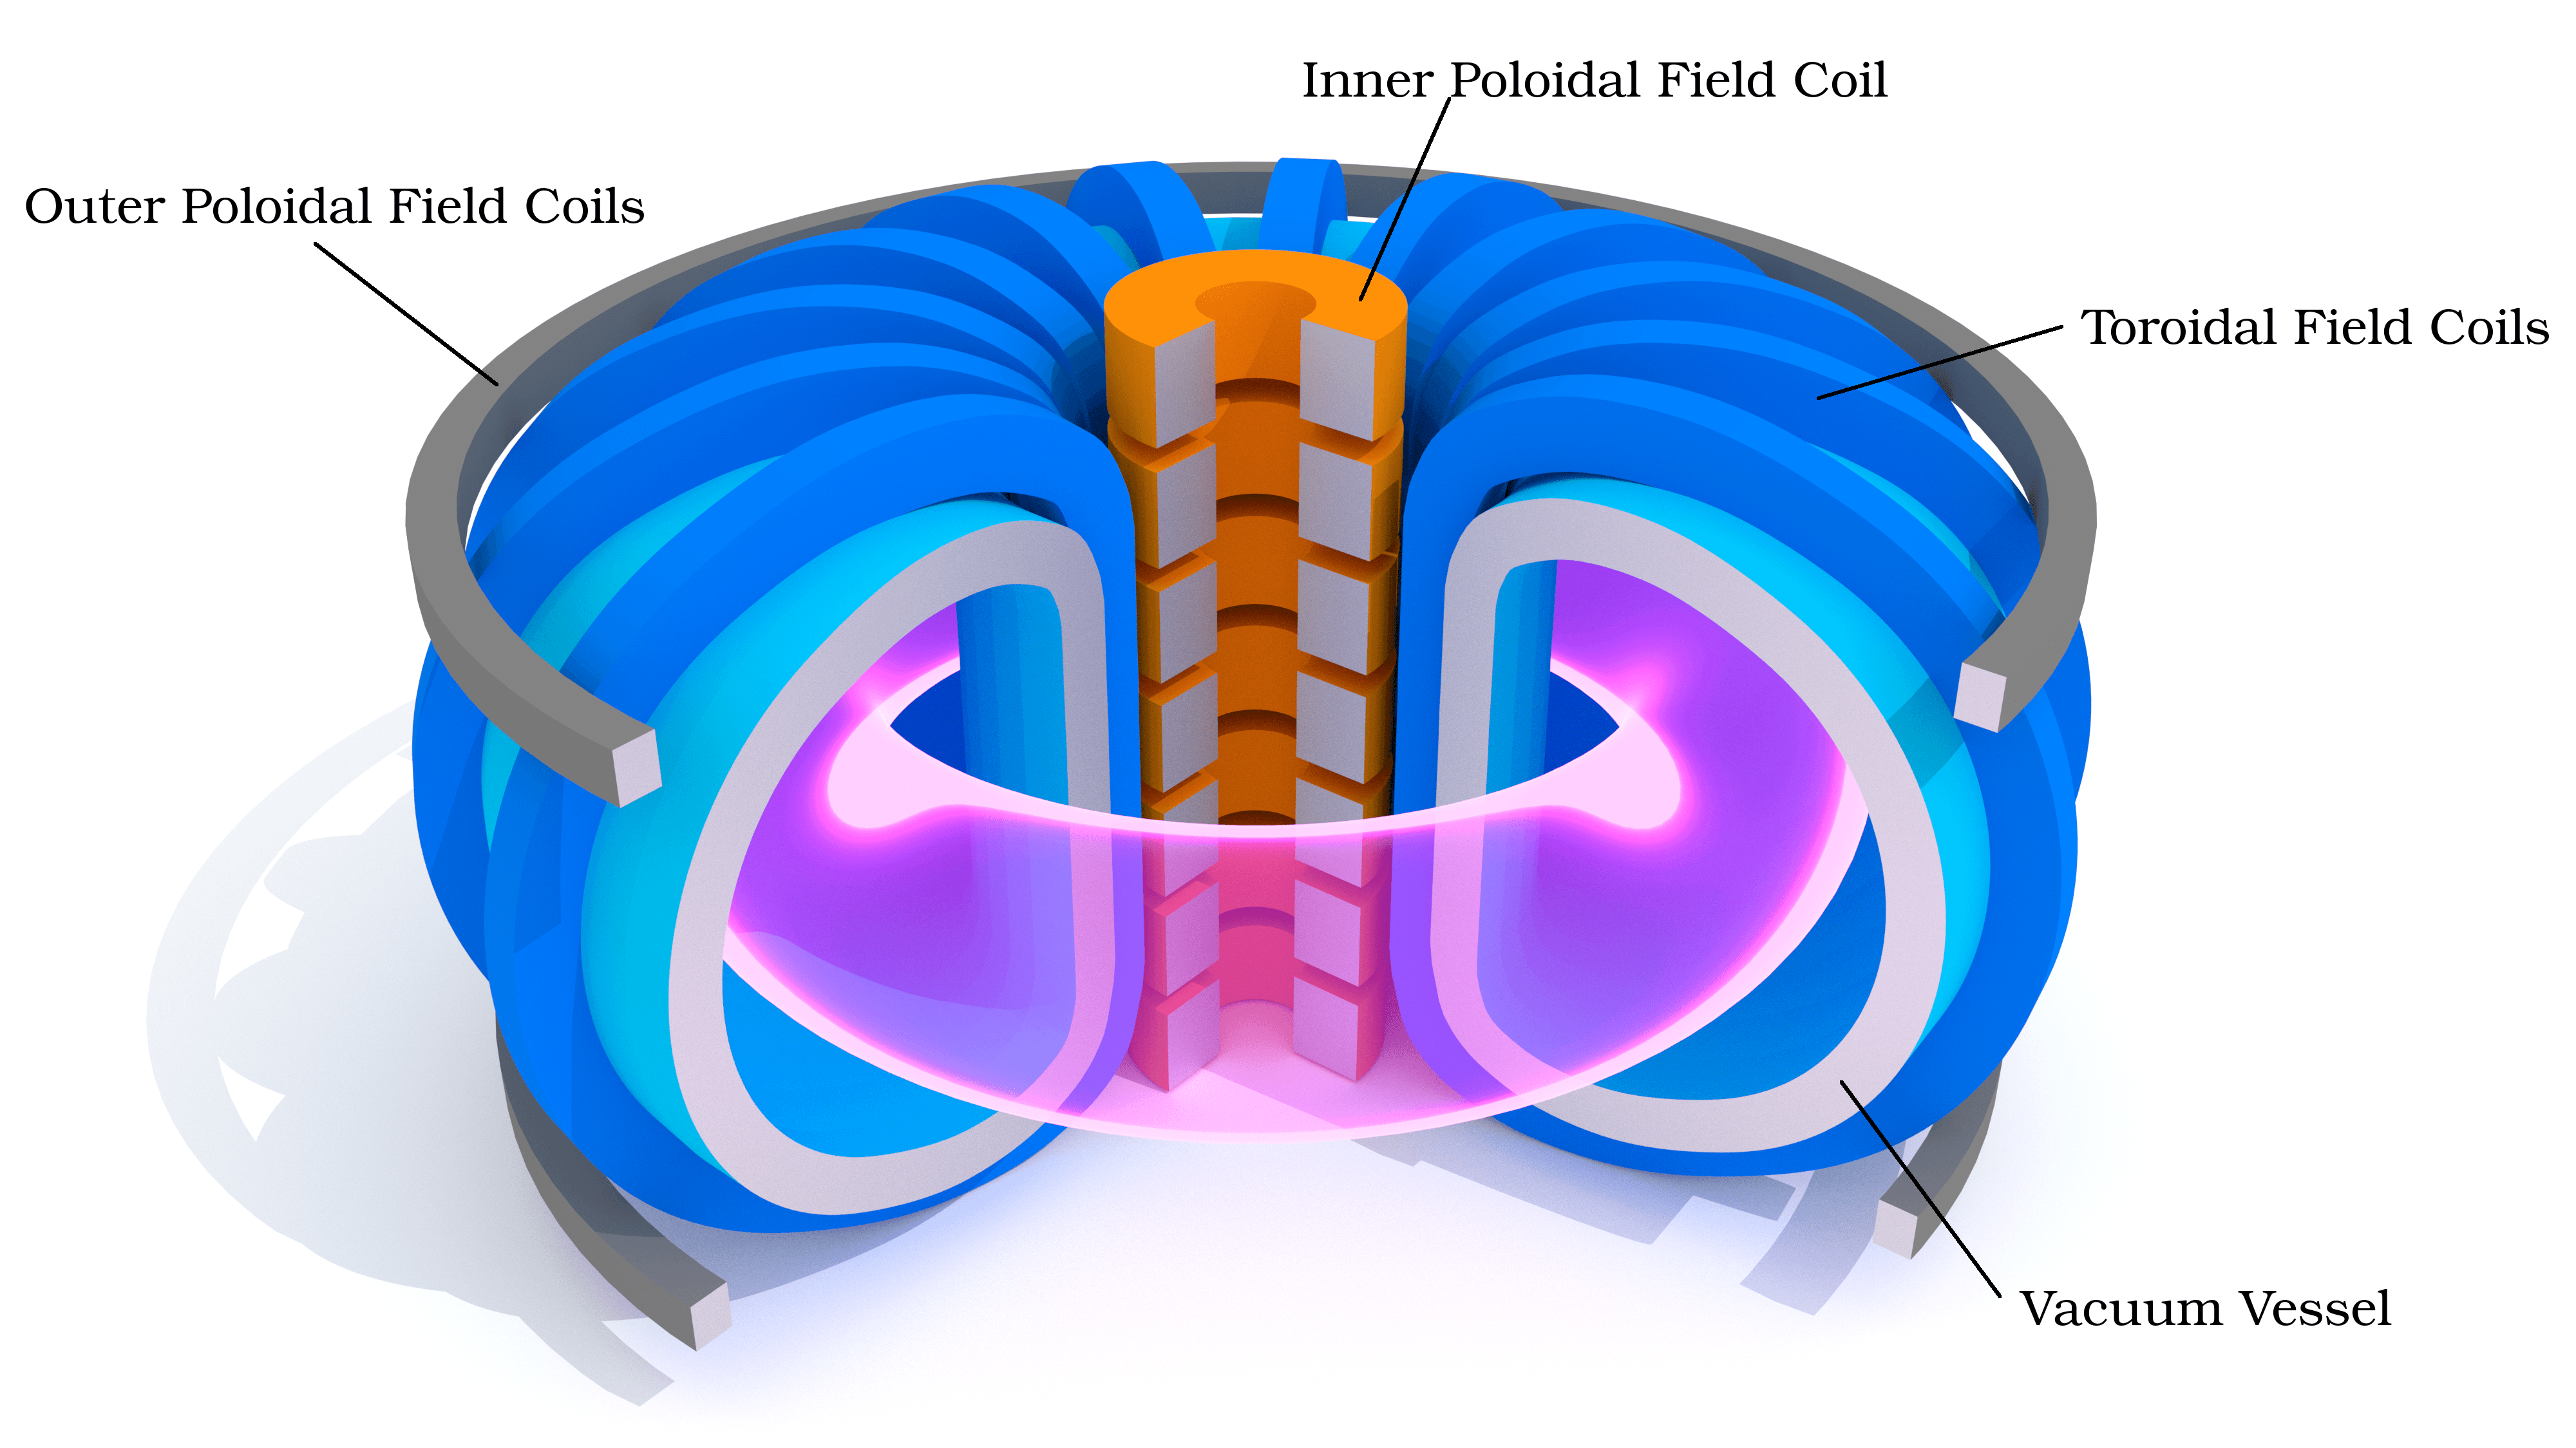
\includegraphics[width=0.8\linewidth]{Schematic-of-a-tokamak.png}
\caption{A schematic view of a tokamak-type fusion reactor.} 
\label{fig:tokamak}
\end{figure}

Regarding the fuel of an MCF reactor, any two light enough elements could in theory be fused. 
However, from a fuel-economical point of view, the deuterium-tritium reaction 
\begin{align}
^2_1\rm{H} ~+~ ^3_1\rm{H} ~\rightarrow~ ^4_2\rm{He} ~+~ ^1_0\rm{n} ~+~ 17.58 ~\rm{MeV}
\label{Eq:D-T-reaction}
\end{align}
is considered one of the most favourable. 
Deuterium can be refined easily out of hydrogen extracted from seawater, while tritium can be produced through transmutation from lithium as
\begin{align}
^6_3\rm{Li} ~+~ ^1_0\rm{n} ~\rightarrow~ ^4_2\rm{He} ~+~ ^3_2\rm{H} ~+~ 4.80  ~\rm{MeV}
\end{align}
using the neutrons released from either a fission or fusion reactor. 
There are plans for using specific "breeding" structures on the inner surfaces of a tokamak for producing tritium \textit{in situ} \cite{giancarli2012overview}.


% ---------------------------------------------------------------------------------------------------
\section{Plasma Facing Components in Modern \& Future Tokamaks}
% ---------------------------------------------------------------------------------------------------

The extreme conditions contained within a fusion reactor impose strict requirements on the construction materials. 
Energetic neutrons and ions are constantly bombarding the plasma-facing components, causing heating of the reactor vessel and erosion of the walls, potentially hindering the fusion process by contaminating the plasma with heavier atoms. 
In order to protect the vacuum vessel from the intense heat and the erosive effects of plasma particles, the inner walls are covered with a cooled and armoured \textit{blanket}. 
In reactors such as the ITER or the Joint European Torus (JET), the blanket is often covered with beryllium \cite{raffray2012overview}, chosen due to its superior plasma contamination properties.

Located usually at the top or bottom of a tokamak, the \textit{divertor} is a device used for on-line removal of fusion products and impurities from the plasma.
Positioned at a intersection of magnetic field lines, the plasma-facing surfaces of the divertor are subject to even more extreme particle bombardment than those of the blanket.
For instance, the vertical targets of the ITER divertor, visible in Fig. \ref{fig:ITERslice}, are expected to receive heat fluxes of up to 20 MW/m$^2$ \cite{Iter1234Divertor}, implying that the material should both be able to withstand high temperatures and have excellent heat transfer properties.

\vspace{35mm}
\begin{figure}[!ht]
\center
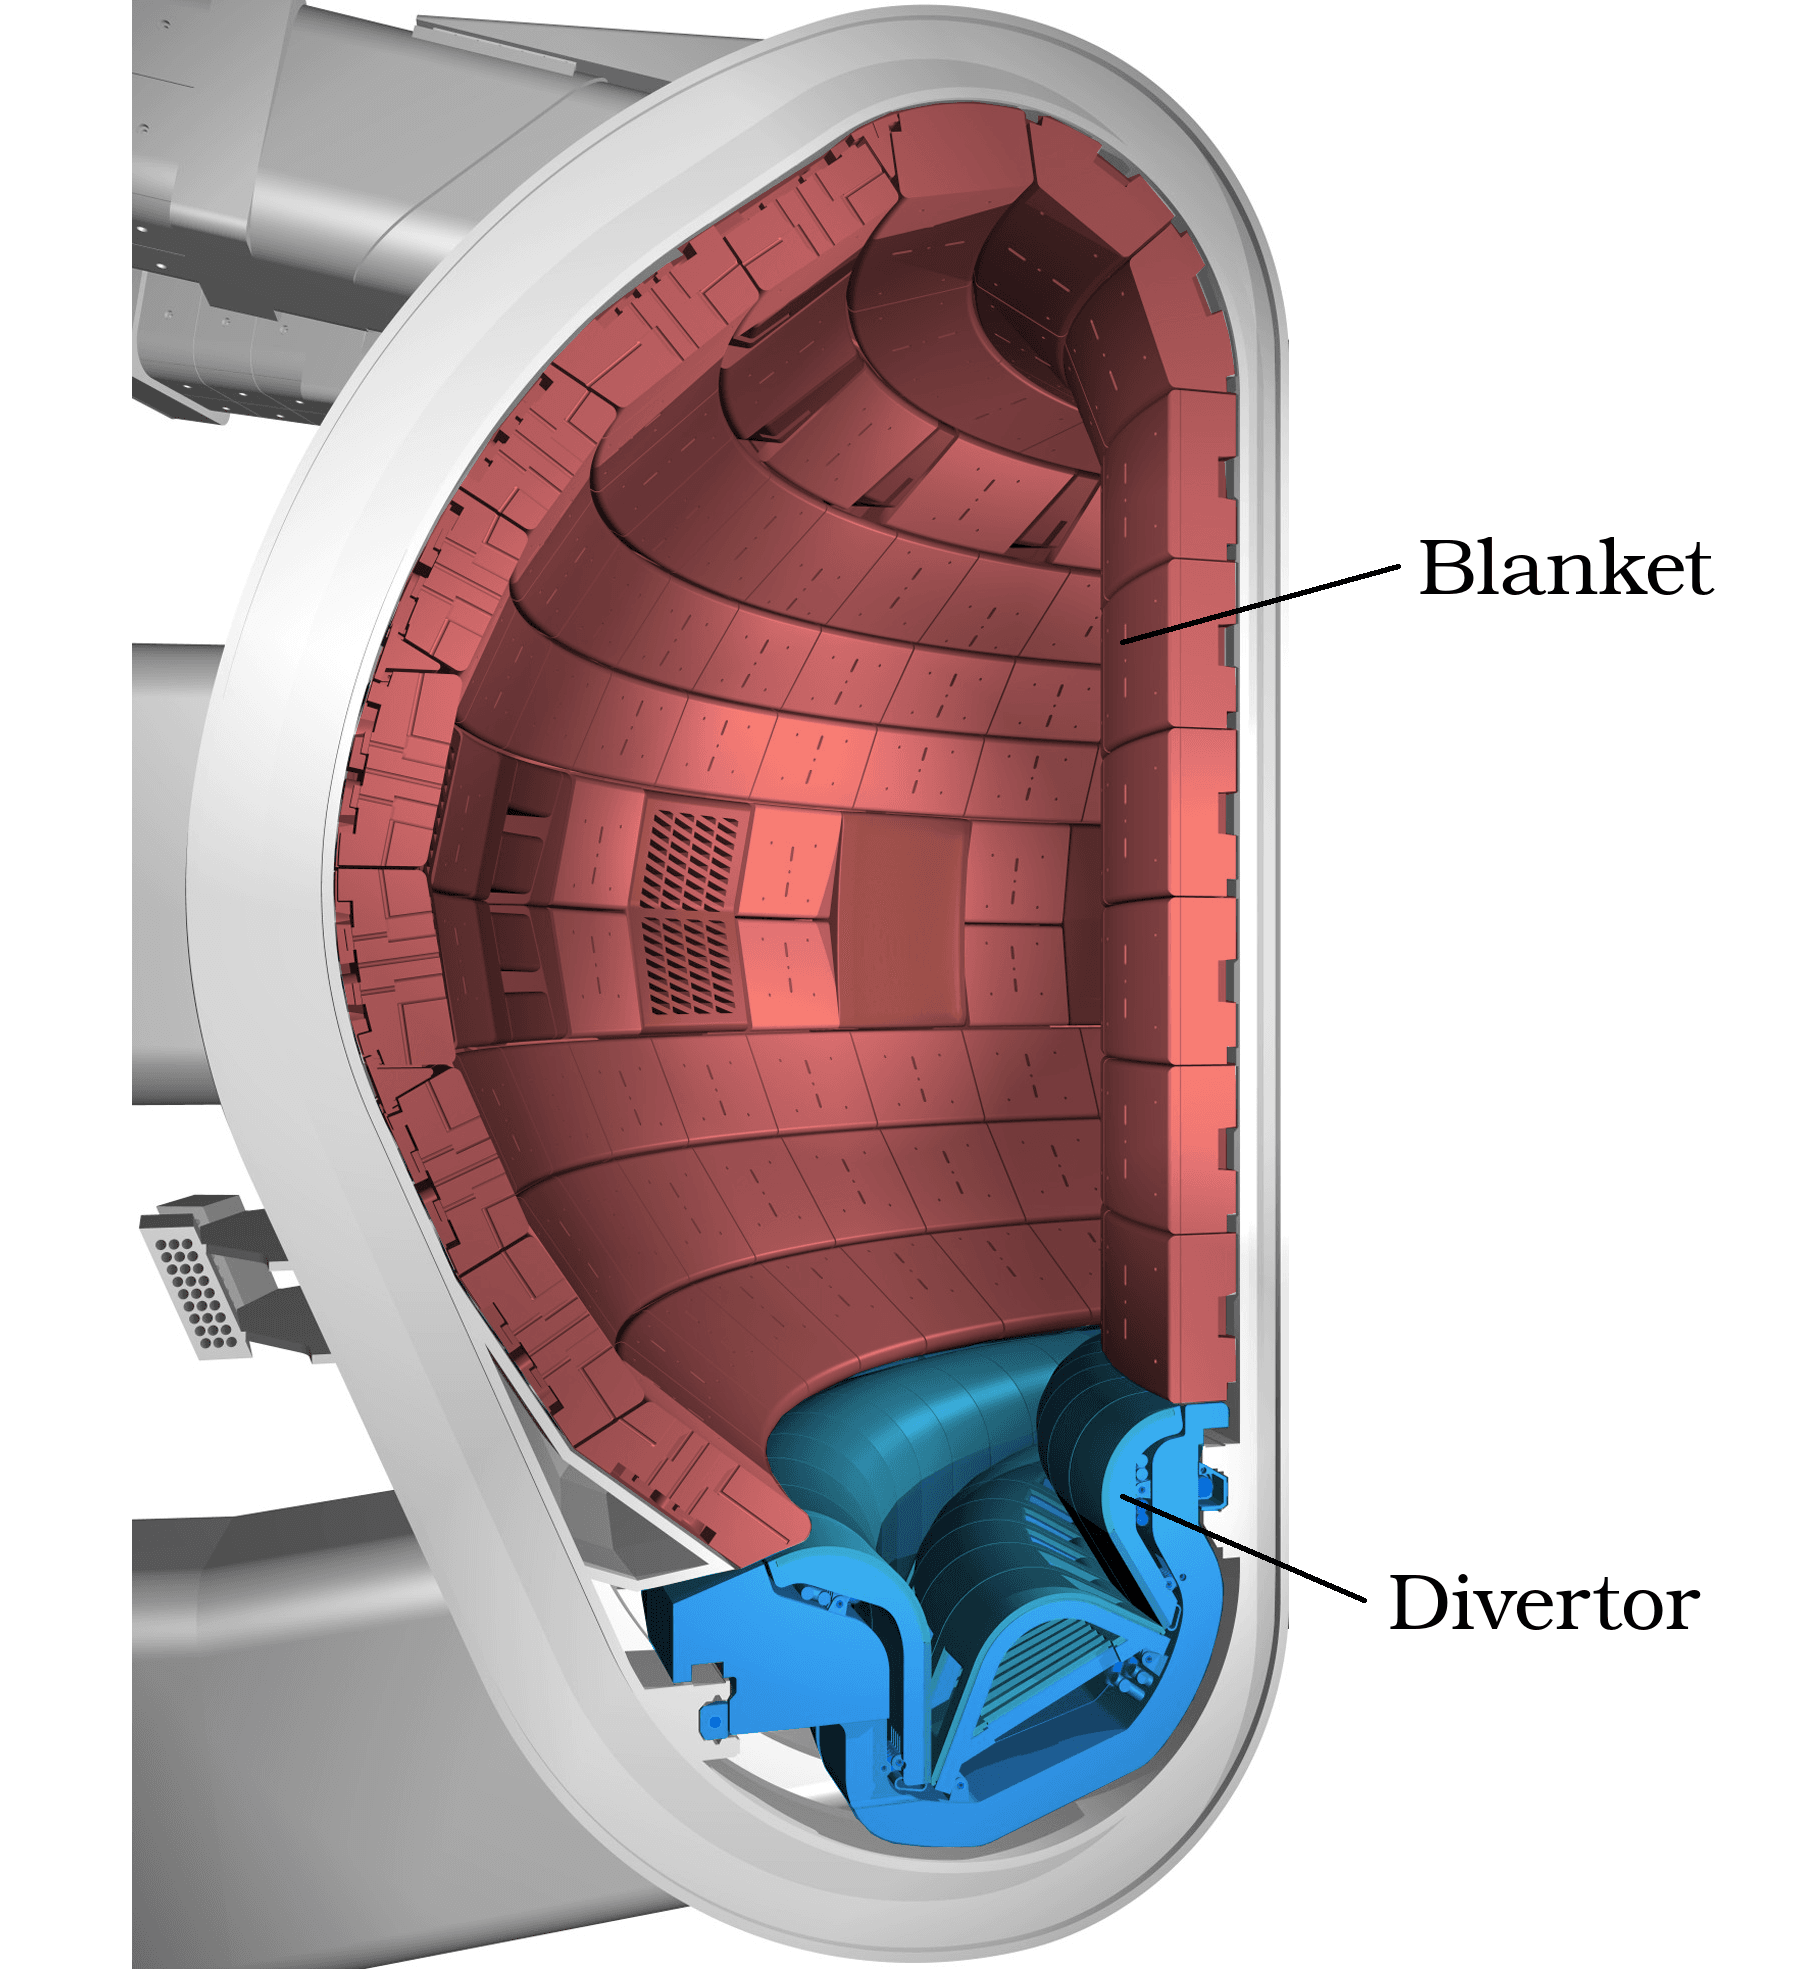
\includegraphics[scale=0.1]{vacuumvessel_edited.png}
\caption{A section of the ITER tokamak with the plasma facing components highlighted. Source: Adapted from \cite{ITERCrossSection}}
\label{fig:ITERslice}
\end{figure}

% ---------------------------------------------------------------------------------------------------
\section{Hydrogen Retention in Tungsten}
% ---------------------------------------------------------------------------------------------------
The armour material of choice for the ITER divertor is tungsten (W) \cite{PITTS2013S48}.
The metal, named after the Swedish word for "heavy stone", is recognized for having the highest melting point of all metals (3695 K) and a hardness superior to that of most steels. 
It also has a thermal conductivity of 173 W/(m·K), equaling around twice that of iron and half that of copper. 
In its structurally most stable form, W has a body-centered-cubic (BCC) crystal structure, with a lattice constant of 3.165 \AA.
Due to its small atomic size, hydrogen is soluble to at least some degree in most transition metals, including tungsten \cite{smith1934occlusion, frauenfelder1969solution}.
The equilibrium position for hydrogen in a perfect W lattice is at the tetrahedral interstitial position (TIS), shown as black dots in Fig. \ref{Fig:bcc}. 

At temperatures $T > 0$ K, any real crystalline materials will contain some amount of crystallographic defects, the most common which are visualized in Fig. \ref{Fig:defect_types}. 
The number of these defects increases with the temperature and as the result of irradiation. 
Defects, being disruptions in the periodicity of a lattice, cause an increase in the potential energy of the atomic system. 
\begin{figure}[!ht]
\center
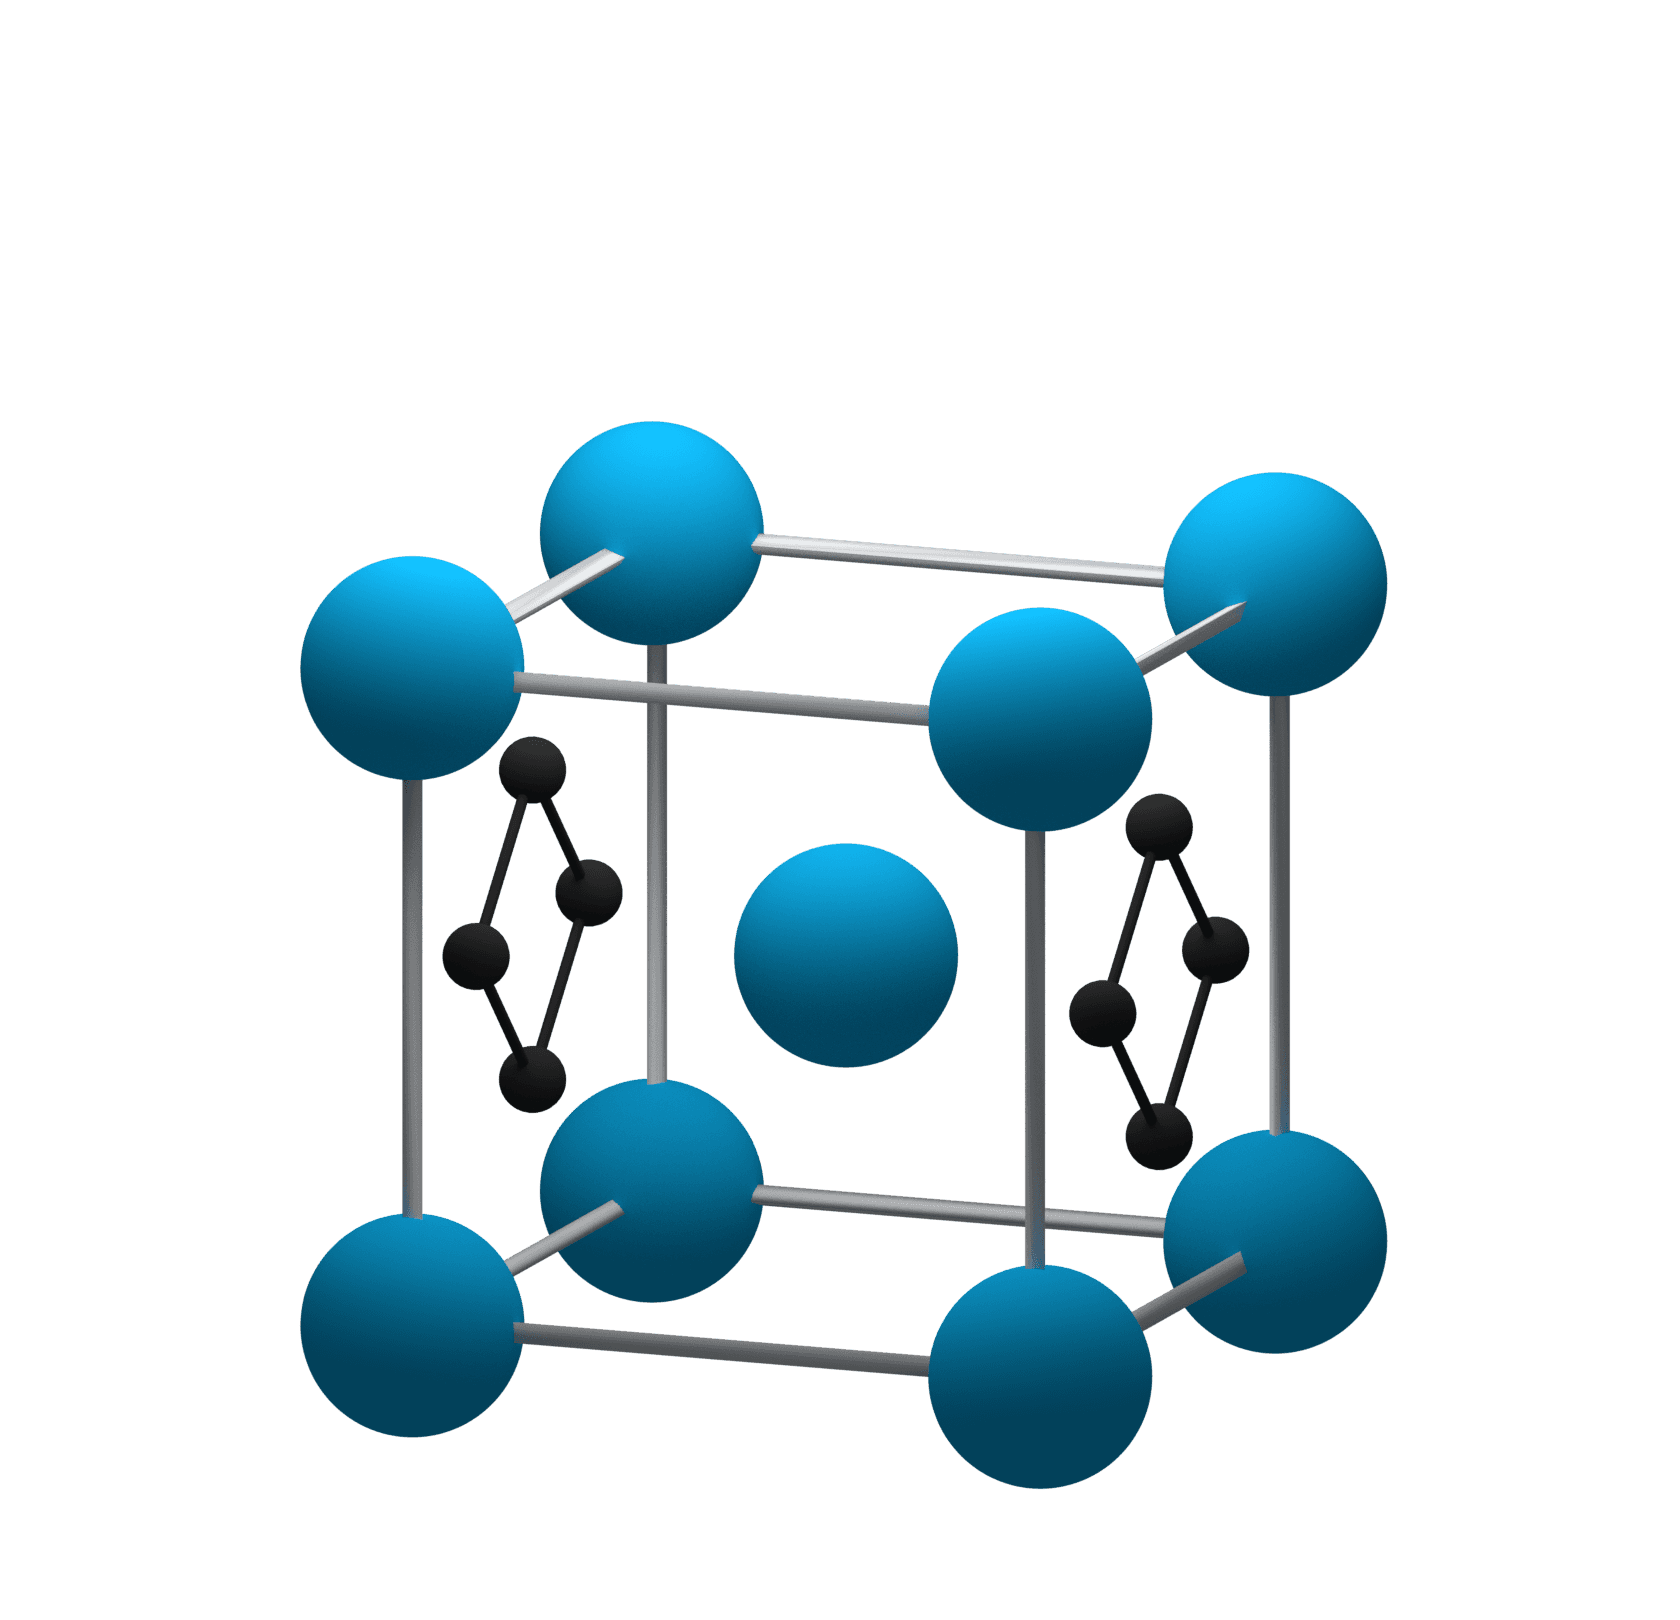
\includegraphics[width=0.3\linewidth]{bcc_render.png}
\caption{The BCC crystalline structure (atoms in blue). Shown in black are 8 out of 24 tetrahedral interstitial positions around the central atom.}
\label{Fig:bcc}
\end{figure}
In a W-H system, formed, e.g. by placing a tungsten object under a hydrogen atmosphere, H atoms tend to lower the system energy by binding to defects. 
E.g. in the case of a vacancy, the empty lattice site leaves neighbouring W atoms with dangling bonds to which hydrogen can bind, leading to a net decrease in energy and six hydrogen atoms being strongly trapped to the defect.

\begin{figure}[!ht]
\center
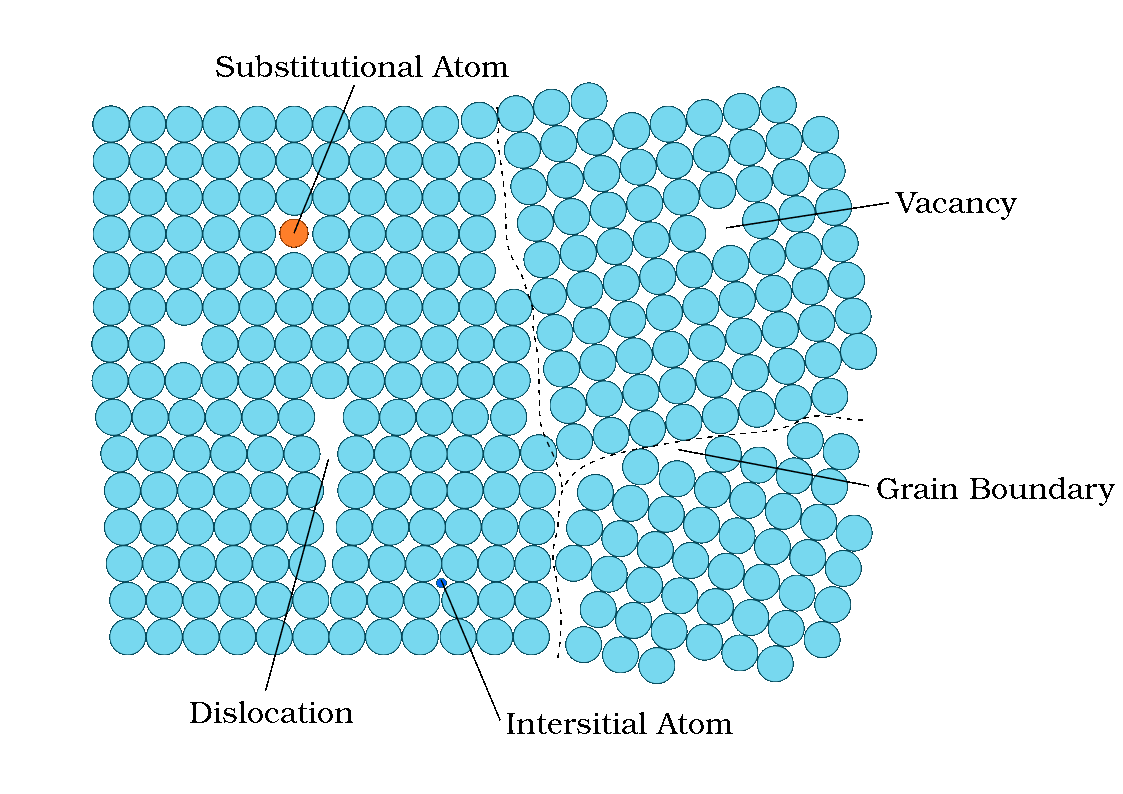
\includegraphics[width=0.76\linewidth]{defect_types.png}
\caption{Various types of crystal defects shown on a 2D lattice}
\label{Fig:defect_types}
\end{figure}


% ---------------------------------------------------------------------------------------------------
\section{Hydrogen Isotope Exchange}
% ---------------------------------------------------------------------------------------------------

The isotopes of a chemical element are essentially variations of the same element, differing in the number of neutrons and thus also atomic mass. 
Since all isotopes of a specific element share the same number of protons and electrons, they can be considered chemically indistinguishable. 
The difference in atomic mass can, nonetheless, present itself as a change in the reaction rates of chemical and thermodynamic processes when an atom is replaced by its isotope. 
Known as the \textit{kinetic isotope effect}, this involves lighter isotopes generally reacting faster than their heavier counterparts \cite{atkins2006atkins}.

In the case of hydrogen, there are three naturally occurring isotopes, protium (H), deuterium (D) and tritium (T). 
In contrast to the vast majority of elements, the relative differences in mass between these three isotopes are notably extreme; D ($m_{\text{D}}=2.014102$ u) and T ($m_{\text{T}}=3.016049$ u) have masses of just over two and three times that of H ($m_{\text{H}}=1.007825$ u). 
These mass differences result in, e.g. the isotopes having noticeably different diffusion rates.

Out of these three isotopes, tritium is the by far scarcest. 
Having a half-life of only 12.3 years, it is formed only in minuscule amounts in the atmosphere through interactions with cosmic rays.
In fusion reactors, where tritium will be present in relative abundance, the trapping of this radioactive substance into wall materials can over time become a safety issue; although tritium is a low-energy beta emitter and thus not externally harmful to humans, it is easily inhaled, ingested or absorbed through the skin, potentially causing radiation damage to internal organs and tissues \cite{tritiumHealth}.
In addition to the safety concern associated with handling and maintaining tritium infused components, there is also an obvious fuel economical incentive of retrieving the embedded tritium.

The proposed methods of detrapping and extracting hydrogen isotopes from materials typically focus on annealing, i.e. heating and slowly cooling a material, to facilitate the detrapping and diffusion of hydrogen atoms. 
Although the rate of diffusion is proportional to temperature as
\begin{align}
D ~\propto~ \exp\left(-\frac{1}{k_{\text{B}}T}\right)
\end{align}
temperatures of above 700 K are still needed to remove the trapped hydrogen within reasonable timescales \cite{heinola2017long}.

% [Description of the proposed mechanism of isotope exchange]
This can be partly understood by looking at the binding energy $E_{\text{bind}}$. For the $N$th H atom bound to a defect, this is calculated as
\begin{align}
E_{\text{bind}}(N) ~=~ E(N-1) + E_\text{sol} - [ E(N) + E_\text{bulk} ]
\end{align}
where $E_\text{bulk}$ is the total energy of the perfect crystalline system and $E(N)$ is that of a system with a defect containing $N$ H atoms. 
% TODO: add E_bind(N) plot? E.g. Heinola et al. 2010 DFT data
$E_\text{sol}$, on the other hand, is the energy of a W lattice without the defect, but with a solute H atom at a TIS site.
For most defects, $E_{\text{bind}}$ decreases with $N$, i.e. each added atom is more loosely bound than the previous.
When a hydrogen atom gets detrapped and diffuses far enough from its original position in a defect, it is unlikely to return; either it gets trapped in another nearby defect or eventually exits through an open surface.
As the defect empties this way, it grows increasingly difficult and therefore unlikely for the remaining hydrogen atoms to overcome the $E_{\text{bind}}$ barrier.
In other words, the removal of T from a material slows over time, unless more heat is gradually applied.

Annealing performed under a H$_2$ atmosphere or alternatively under a bombardment of H plasma has, however, been experimentally shown to reduce annealing time or alternatively enable the annealing to be performed at lower temperatures \cite{alimov2011hydrogen, roth2013hydrogen, barton2014deuterium, ahlgren2019hydrogen}.
The mechanism at play here supposedly works by keeping the number of hydrogen atoms bound to a defect constant.  
As a tritium atom now leaves the defect, its place is soon taken by a close-by protium atom, resulting in the low-$E_{\text{bind}}$ states being kept occupied even as the T-removal progresses.
Since hydrogen atoms are assumed to move around somewhat in the defect, the low-$E_{\text{bind}}$ states are shared between the new H atoms and the T atoms remaining in the defect.

